\subsection{Cubrimientos pares}
\begin{definicion}
Sea \(p : \tilde{X} \to X\) una funcion continua sobreyectiva. El abierto \(U
\subseteq X\) se dice \textbf{parmente cubierto} por \(p\) si existe
\(\{V_\alpha\}_{\alpha \in \Lambda},\ \Lambda \subseteq \mathbb N\) tal que
\[ p^{-1} (U) = \bigcup_{\alpha \in \Lambda} V_\alpha \]
Donde \(\{V_\alpha\}\) es una familia disjunta de abiertos, tal que
\(\forall \alpha \in \Lambda, p \mid_{\alpha}\) es homeomofo sobre \(U\).

Si para todo \(x \in X\) existe dicha vecindad \(U\) que cumpla lo
anterior, se dira que \(\tilde{X}\) es un \textbf{espacio cubrimiento} de \(X\)
y que \(p\) es un \textbf{cubrimiento par}.
\end{definicion}

Un ejemplo simple de espacio cubrimiento y cubrimiento par es \(p :
\mathbb R \to S^1,\ p(t) := e^{2 \pi \imath t}\). Este es claramente
sobreyectivo y continuo, escogiendo dos abiertos ejemplares como \(U =
S^1 - \{(1,0)\}\) y \(V = S^1 - \{(-1,0)\}\), es claro que
\[
    p^{-1} (U) = \bigcup_{n \in \mathbb Z} (n, n+1)
    \qquad p^{-1} (V) = \bigcup_{n \in \mathbb Z} (n - \frac 1 2, n + \frac 1
    2 )
\]
Donde estas familias de conjuntos son disjuntos y restringidos a cada
uno se tiene la inyectividad requerida.

A priori el cubrimientos par es independiente de los caminos que tengamos
en \(X\), queremos ver si podemos reflejar la informacion importante de
los caminos en \(\tilde{X}\).
\begin{figure}[h]
  \centering
  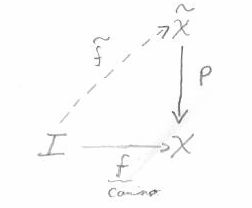
\includegraphics[scale=0.5]{./imagenes/lifting-path-diagrama.png}
\end{figure}
Para esto construiremos \(\tilde f : I \to \tilde X\) el cual cumpla \(p
\circ \tilde f = f \), donde \(\tilde f\) sera nuestro representante en
el espacio cubrimientos de estos caminos. Veremos tambien que bajo
hipotesis sensatas, este \(\tilde f\) es unico y refleja informacion
homotopica. Para esto necesitamos desarrollar algunos teoremas previos.
\begin{lema}[Numero de Lebesgue] \label{thm:lebesgue-number-lema}
  Sea \(\mathcal A\) un cubrimiento del espacio metrico \((X,d)\). Si
  \(X\) es compacto, entonces existe \(\delta > 0\) tal que para todo
  subconjunto de \(X\) teniendo diametro menor que \(\delta\), existe un
  elemento de \(\mathcal A\) conteniendolo.
\end{lema}
\begin{proof}
  Supongamos que \(X \not \in \mathcal A\), pues si no trivialmente el
  teorema se cumple \(\forall \delta > 0\). Por compacidad de \(X\)
  existe una coleccion \(\{A_1,\dotsc,A_n\} \subset \mathcal A\) que
  cubre a \(X\), definamos a los conjuntos \(C_i = X - A_i,\ \forall i
  \in [1,n]\) y a la funcion \(f : X \to \mathbb R\) definida por
  \[ f(x) := \frac 1 n \sum_{i=1}^{n} d(x, C_i) \]
  i.e. la distancia promedio de \(x\) a \(C_i\). Notemos que \(\forall x,\
  f(x) > 0\), pues para \(x \in A_i \subseteq X\), por ser \(A_i\) un
  abierto, existe \(\epsilon > 0\) tal que \(B(x,\epsilon) \subset A_i\)
  y por tanto \(d(x, C_i) \geq \epsilon\) que implica  \( f(x) \geq \frac
  \epsilon n > 0\).

  Por otro lado \(f\) es una funcion continua sobre \(X\), un compacto,
  por lo tanto alcanza un minimo; a este le denotaremos como nuestro
  \(\delta\). Probaremos que este cumple el requerimiento, sea \(B
  \subset X\) subconjunto abierto de diametro menor que \(\delta\), sea
  \(x \in B\) arbitrario, el cual tiene tiene una vecindad contenida en
  \(B\) de diametro menor a \(\delta\). Dado que
  \[\delta \leq f(x) \leq d(x, C_m) \qquad
      d(x, C_m) := \max_{i \in [1,n]} d(x, C_i)\]
  Esto nos dice que dado \(\delta \leq d(x, C_m)\), existe una vecindad
  de al menos diametro \(\delta\) que contiene a \(x\) en \(X - C_m = A_m\).
\end{proof}
\begin{definicion}[Levantamiento de \(f\)]
  Sea \(p : \tilde X \to X\) un mapeo. Si \(f : W \to X\) es un mapeo
  continuo, un levantamiento de \(f\) es una funcion \(\tilde f : W \to
  \tilde X\) tal que \(p \circ \tilde f = f\).
\end{definicion}
Ver que la definicion es mucho mas general que lo que pediamos al
diagrama. Usualmente \(W = [0,1]\) pues estudiaremos los caminos sobre
\(X\). Veremos a continuacion teoremas de como se reflejan los caminos
y las homotopias en el espacio cubrimiento de \(X\).
\begin{teorema}\label{thm:lifting-theorem}
  Sea \(p : \tilde X \to X\) un cubrimiento par y \(x_0 \in X\). Fijemos
  algun \(\tilde x _0 \in \tilde X\) tal que \(p(\tilde x _0) = x_0 \).
  Para cualquier camino \(f : [0,1] \to X\) que comience en \(x_0\), existe
  un unico camino levantamiento \(\tilde f : [0,1] \to \tilde X\) tal que
  \(\tilde f (0) = \tilde x _0\)
\end{teorema}
\begin{proof}
  Para todo punto de \(x \in X\), existe una vecindad \(U_x\) que es
  cubierta parmente, por tanto \(\bigcup_{x \in X} U_x\) es cubrimiento de
  \(X\). Por otro lado, tenemos que \( [0,1] \subset f^{-1} (\bigcup_{x
  \in X} U_x)\); por el Teorema \ref{thm:lebesgue-number-lema}, podemos
  elegir \(s_0,\dotsc,s_n \in [0,1]\) tal que \(f([s_i, s_{i+1}])\) este contenido
  en algun \(U_x\). Definiremos \(\tilde f\) inductivamente.

  Primero declaremos \(\tilde f (0) = \tilde x _0\). Luego, suponiendo
  que \(\tilde f (s)\) esta definido para \(s \in [0, s_i]\), se
  define a \(\tilde f \) en \([s_i, s_{i+1}]\) de la siguiente forma.
  Dado que para algun \(x \in X\),
  \[f ([s_i, s_{i+1}]) \subseteq U_x \quad \land \quad \exists
    \{V_\alpha\}_{\alpha \in \Lambda},\ \bigcup_{\alpha \in \Lambda}
    V_\alpha = p^{-1} (U_x)\]
  debe de existir \(\alpha \in \Lambda\) tal que \(\tilde f (s_i) \in
  V_\alpha\); a este, le denotaremos \(V_0\). Dado que \(p \mid_{V_0}\) es un
  homeomorfismo, definimos a \(\tilde f (s)\) en \([s_i, s_{i+1}]\) por
  \begin{equation}
  \tilde f (s) = (p \mid _{V_0})^{-1} (f(s))\label{eq:tilde-f-inductiva}
  \end{equation}
  El cual es continuo en \([s_i, s_{i+1}]\) en virtud del lema del
  pegamiento y bien definido por ser \((p \mid _{V_0})^{-1} \) homeomorfismo.

  Para ver la unicidad, se probara inductivamente. Supongamos que existe
  otro \(\hat{f}\) levantamiento par de \(f\) que tambien
  comienza en \(x_0\), ie \(\hat{f} (0) = \tilde x _0 = \tilde f
  (0)\). Supongamos que que \(\forall s \in [0, s_i],\ \hat{f}
  (s) = \tilde f (s)\), dado que \(\tilde f\) esta definida por
  \eqref{eq:tilde-f-inductiva}, \(\hat f\) debe ser
  eventualmente diferente a la definicion \eqref{eq:tilde-f-inductiva},
  pero
  \[\hat f (s_i) = \tilde f (s_i) \in V_0\]
  con \([s_i, s_{i+1}]\) conexo y la familia \(\{V_\alpha\}\)
  es disjunta, obliga\footnote{Funciones continuas mapean conjuntos
    conexos a conexos} a que \(\hat f [s_i, s_{i+1}] \subset
  V_0\). Dado que es un levantamiento, debe de cumplirse que
  \[\forall s \in [s_i, s_{i+1}],\ p \circ \hat f \, (s) =
    f(s) = p \circ \tilde f \, (s) \]
  \[ \iff p ( \hat f (s)) = p ((p \mid_{V_0})^{-1} (f (s)))\]
  \[ \implies \hat f (s) = (p \mid_{V_0})^{-1} (f (s)), \quad \forall s
      \in [s_i, s_{i+1}]\]
  siendo esta la unica posible definicion, pues de haber otra,
  contradeceria que \((p \mid_{V_0})\) es un homeomorfismo (mapeo
  unico), por tanto se obliga a que \( \hat f = \tilde f\)
\end{proof}
\begin{corolario}
  Sea \(p : \tilde X \to X\) un cubrimiento par tal que \(p(\tilde x _0)
  = x_0 \) para algun \(\tilde x _0 \in \tilde X\). Para cualquier
  funcion continua \(F : I \times I \to X\) tal que \(F(0,0) = x_0\), tiene una
  unica funcion levantamiento continua \(\tilde F : I \times I \to
  \tilde X\) que cumpla \(\tilde F (0,0) = \tilde x_0\)
\end{corolario}
\begin{proof}
  Lo unico diferente con el teorema \ref{thm:lifting-theorem} es que
  tomamos \(I \times I\) que sigue siendo compacto. Podemos aplicar el
  teorema anterior primero definiendo \(\tilde F\) en \(0 \times I\) y
  luego en \(I \times 0\), luego escogiendo subdivisiones de \(I \times
  I\)
  \[ s_0 < s_1 < \dotsc < s_m \]
  \[ t_0 < t_1 < \dotsc < t_n \]
  construidos de manera analoga al teorema anterior. Luego podemos
  definir \(\tilde F\) inductivamente ``por filas'' y luego ``por
  columnas'', ya que aun mantenemos la invariante de preservar punto en
  comun entre rectangulos \([s_{i-1}, s_i] \times [t_{i-1}, t_i]\).
\end{proof}
\begin{definicion}
  Sea \(p : \tilde X \to X\) un cubrimiento par; sea \(x_0 \in X\).
  Escojamos \(\tilde x _0 \in \tilde X\) tal que \(p(\tilde x _0) =
  x_0\). Dado un elemento \([f] \in \pi (X, x_0)\), sea \(\tilde f\) el
  levantamiento (unico) de \(f\) a un camino en \(\tilde X\) que
  comienza en \(\tilde x _0\). Definamos \(\phi ([f]) = \tilde f (1)\) del
  \(\tilde f\) asociado a \(f\) anteriormente. Entonces \(\phi\) es bien
  definido como mapeo de conjunto
  \[ \phi : \pi (X, x_0) \longrightarrow p^{-1} (x_0)\]
  llamando a \(\phi\) el \textbf{correspondiente levantamiento derivado}
  del mapeo cubrimiento par \(p\).
\end{definicion}
La definicion anterior intuitivamente ``desenrolla'' los ciclos del
grupo fundamental \(\pi (X,x_0)\) y ve donde terminan vistos sobre
\(\tilde X\).
\begin{teorema}
  Sea \(p : \tilde X \to X\) un cubrimiento par, sea \(p (\tilde x _0) =
  x_0\). Si \(\tilde X\) es arco-conexo entonces el correspondiente
  levantamiento \(\phi : \pi (X, x _0) \to p^{-1} (x)\) es sobreyectivo.
  Mas aun, si \(\tilde X\) es simplemente conexo, este es biyectivo.
\end{teorema}
Usualmente queremos que \(p^{-1} (x)\) no sea simplemente un conjunto,
queremos poder dotarle de estructura de grupo. En caso de \(\tilde X\)
ser arco-conexo, lo que estamos haciendo realmente es estudiar un
subgrupo de \(X\) a traves de \(p^{-1}(x_0) \subseteq \tilde X\).
\begin{proof}
  Demostracion estandar de sobreyectividad en caso de ser \(\tilde X\)
  arco-conexo. Para \(\tilde x _1 \in p^{-1} (x_0)\) arbitrario, existe
  \(\tilde f\) camino entre \(\tilde x _0 \) a \(\tilde x _1\) por
  arco-conexidad. Definimos \(f := p \circ \tilde f\), el cual es un
  camino \(f : I \to X\) que cumple \(\phi ([f]) = \tilde x _1\) por
  definicion.

  En caso de ser \(\tilde X\) simplemente-conexo, veremos solo la
  inyectividad. Sean \([f],[g] \in \pi (X, x_0)\) tales que \(\phi([f])
  = \phi([g])\), mostraremos que \([f] = [g]\). Sean \(\tilde f, \tilde
  g : I \to \tilde X\) los levantamientos respectivos que comienzan en
  \(\tilde x _0\). Dado que \(\phi([f]) = \tilde f (1) = \tilde g (1) =
  \phi([g])\) y la simple-conexidad de \(\tilde X\), existe \(\tilde F :
  I \times I \to \tilde X\) homotopia \(\tilde f, \tilde g\). Luego \(p
  \circ \tilde F : I \times I \to X \) es una homotopia entre \(f, g\),
  por tanto \([f] = [g]\)
\end{proof}
Ahora podemos plantearnos un ejemplo clasico, ver el grupo fundamental
de \(S^1\). Utilizaremos el teorema anterior para proponer un
cubrimiento tal que \(\tilde X\) sea simplemente conexo y que pueda
preservar la estructura de grupo para ser estudiado bajo ese lente.
\begin{teorema}
  \(\forall x_0 \in S^1,\ \big( \pi (S^1,x_0), * \big)\) es isomorfo a
  \((\mathbb Z, +)\)
\end{teorema}
\begin{proof}
  Dado que \(S^1\) es arco-conexo, basta probar que este teorema es
  cierto para algun \(x_0\) en \(S^1\). Sea \(p : \mathbb R \to S^1,\
  p(t) := (\cos 2 \pi t, \sin 2 \pi t)\) el cual es fue visto anteriormente
  que es un cubrimiento par. Sea \(\tilde x _0 = 0\) y \( p(\tilde x _0) =
  (1,0) =: x_0 \in S^1\). Por ser \(\mathbb R\) simplemente conexo, se
  tiene que el levantamiento correspondiente \(\phi : \pi (S^1, x_0) \to
  p^{-1} (x_0)\) es biyectivo, donde
  \[ p^{-1} (1,0) = \{t \in \mathbb R \mid (\cos 2 \pi t, \sin 2 \pi t)
    = (1, 0) \} = \mathbb Z \]

  Para probar que ademas es homomorfismo, se toman \([f], [g] \in \pi
  (S^1, x_0)\) arbitrarios y \(\tilde f, \tilde g\) sus correspondientes
  levantamientos tales que \(n := \tilde f (1) = \phi ([f]),\ m :=
  \tilde g (1) = \phi ([g])\). Se define el camino
  \begin{align*}
    \tilde{\tilde g} : I &\longrightarrow \mathbb R \\
    s &\longmapsto n + \tilde g (s)
  \end{align*}
  Puesto que \(p(n + x) = p(x)\) por periodicidad, se cumple que
  \[ p \circ \tilde{\tilde g} (x) = p (n + \tilde g (x)) = p (\tilde g
    (x)) = g (x) \]
  Por tanto \(\tilde{\tilde g}\) es el levantamiento de \(g\) para
  \(\tilde x_0 = n\) (en vez de \(\tilde x_0 = 0\)). Luego el producto
  \(\tilde f * \tilde{\tilde g}\) esta bien definido pues \(\tilde f (1)
  = n = \tilde{\tilde g} (0)\) y es el levantamiento de \(f * g\). Por
  definicion
  \[ \phi ([f] * [g]) = \tilde{\tilde g} (1) = n + m = \phi ([f]) + \phi ([g]) \]
  Por lo que \(\phi\) es un homo-morfismo de grupos.
\end{proof}

\paragraph{Cubrimiento \(p_n : S^1 \to S^1\).} Para testear la intuicion
de que el espacio cubrimiento refleja en el caso comun un subgrupo del
espacio topologico, tomemos el caso
\begin{align*}
  p_n : S^1 &\longrightarrow S^1 \\
  z &\longmapsto z^n
\end{align*}
Este

\begin{teorema}
  Sea \(p : \tilde X _1 \to X_1,\ p' : \tilde X _2 \to X_2 \) dos
  cubrimientos pares, entonces
  \[ p_1 \times p_2 : \tilde X _1 \times \tilde X _2 \to X_1 \times X_2 \]
  Es un cubrimiento par.
\end{teorema}
\begin{proof}
  Para todo \(x_1 \in X_1,\ x_2 \in X_2\), existen \(U_1, U_2\)
  vecindades pares respectivamente tales que son cubiertas por \(p_1,
  p_2\). Denotemos a \(\{V_\alpha^{(1)}\}, \{V_\beta^{(2)}\}\) familias
  de conjuntos tales que
  \[
    \begin{matrix}
      \bigcup_{\alpha} V_\alpha^{(1)} = p_1^{-1} (U_1) &
      \bigcup_{\alpha} V_\alpha^{(2)} = p_2^{-1} (U_2)
    \end{matrix}
  \]
  \[ \bigcup_{\alpha, \beta} V_\alpha^{(1)} \times V_\beta^{(2)} = (p_1
    \times p_2)^{-1} (U_1 \times U_2)\]
  Donde la restriccion a un \(V_{\bar{\alpha}}^{(1)} \times
  V_{\bar{\beta}}^{(2)}\) arbitrario en \(p_1 \times p_2\) obtiene un
  homeomorfismo en virtud de las componentes.
\end{proof}
